

\documentclass[xcolor=dvipsnames,10pt]{beamer}


\mode<presentation>
{
  \usetheme{Berlin}  
  \usecolortheme{seahorse}
  \setbeamercovered{transparent}

}


\usepackage[english]{babel}
\usepackage{amsmath, amssymb,color,url,amsthm,amsfonts}
\usepackage{amstext}
\usepackage{graphicx}
\usepackage{wrapfig}
\usepackage{multimedia}
\usepackage{verbatim}
\usepackage{hyperref}
\usepackage[absolute,overlay]{textpos}
\usepackage{algorithm,algorithmic}


\usepackage{bibentry}

\beamertemplatenavigationsymbolsempty

\setbeamertemplate{headline}{}
\setbeamertemplate{footline}
{
  \leavevmode%
  \hbox{%
  \begin{beamercolorbox}[wd=.333333\paperwidth,ht=2.25ex,dp=1ex,center]{author in head/foot}%
    %\usebeamerfont{author in head/foot}\insertshortauthor~~{\insertshortinstitute}{}
  \end{beamercolorbox}%
  \begin{beamercolorbox}[wd=.333333\paperwidth,ht=2.25ex,dp=1ex,center]{title in head/foot}%
    %\usebeamerfont{title in head/foot}\insertshorttitle
  \end{beamercolorbox}%
  \begin{beamercolorbox}[wd=.333333\paperwidth,ht=2.25ex,dp=1ex,right]{date in head/foot}%
    \usebeamerfont{date in head/foot}\hspace*{2em}
    \insertframenumber\hspace*{2ex} 
  \end{beamercolorbox}}%
  \vskip0pt%
}

\setbeamertemplate{caption}{\insertcaption}


\usepackage[utf8]{inputenc}
\newcommand{\ds}{\displaystyle}
\newcommand{\R}{{\mathbf R}}
\newtheorem{proposition}[theorem]{Proposition}




\usepackage{times}
\usepackage[T1]{fontenc}
% Or whatever. Note that the encoding and the font should match. If T1
% does not look nice, try deleting the line with the fontenc.


\title[Rice University]  {Multigrid Solver for Laplacian Linear Systems on Power-Law Graphs}
\author[Buras]{\Large\textbf{Eric Buras}\\
\vspace{.15in}
\textit{\normalsize Adviser: Dr. Matthew Knepley}}

\date{March 25, 2016}
\institute[]{Rice University \\ Department of Computational and Applied Mathematics}



% If you have a file called "university-logo-filename.xxx", where xxx
% is a graphic format that can be processed by latex or pdflatex,
% resp., then you can add a logo as follows:

%\pgfdeclareimage[height=1cm]{ricelogo.png}{ricelogo.png}
 %\logo{\pgfuseimage{ricelogo.png}}



% Delete this, if you do not want the table of contents to pop up at
% the beginning of each subsection:
%\AtBeginSubsection[]
%{
  %\begin{frame}<beamer>{Outline}
   % \tableofcontents[currentsection,currentsubsection]
 % \end{frame}
%}


% If you wish to uncover everything in a step-wise fashion, uncomment
% the following command: 

%\beamerdefaultoverlayspecification{<+->}


%%%%%%%%%%%%%%%%%%%%%%%%%%%%%%%%%%%%%%%%%%%%%

\begin{document}
 
\begin{frame}
  \titlepage
   %\bibliographystyle{plain}
  %\nobibliography{mastersbib}
  \begin{center}

\includegraphics[width=.3\linewidth]{rice.png}
\end{center}
\end{frame}

%%%%%%%%%%%%%%%%%%%%%%%%%%%%%%%%%%%%%%%%%%%%%
\begin{frame}
\begin{figure}
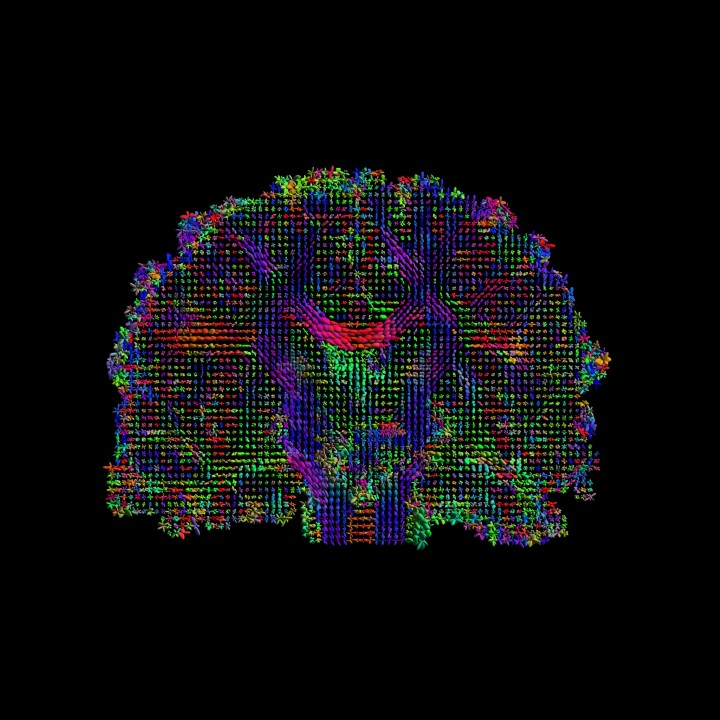
\includegraphics[width=.65\linewidth]{HumanConnectome.png}
\caption{Human brain connectome; coronal view \cite{Toga:2012}}
\end{figure}
\end{frame}
%%%%%%%%%%%%%%%%%%%%%%%%%%%%%%%%%%%%%%%%%%%%%

%\begin{frame}{Outline}
%\tableofcontents
%%  % You might wish to add the option [pausesections]
%\end{frame}





%%%%%%%%%%%%%%%%%%%%%%%%%%%%%%%%%%%%%%%%%%%%%
\section{Introduction}

\begin{frame}{Foundation}
\vspace{.3in}
\textbf{Graph}: $G=(N,E)$ where $N$ is the set of nodes and $E$ is the set of edges.

\begin{figure}
\begin{center}
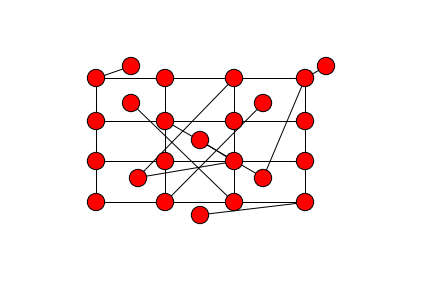
\includegraphics[width = 3.5in]{entiregraph.png}
\end{center}
\end{figure}
\end{frame}



%%%%%%%%%%%%%%%%%%%%%%%%%%%%%%%%%%%%%%%%%%%%%%%%%

\begin{frame}{Foundation}
\vspace{.3in}
Laplacian matrix of $G$:\\
\begin{center}
$L=D-A$\\
\end{center}
$D$: diagonal matrix of node degrees, $A$: adjacency matrix of $G$

\begin{figure}
\begin{center}
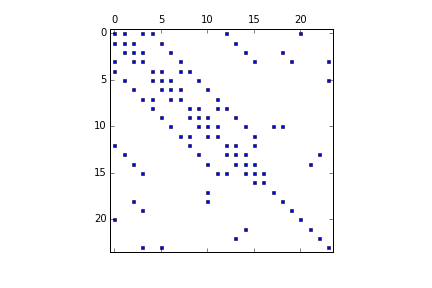
\includegraphics[width = 3.2in]{gridspy.png}
%\caption{Spy plot of the laplacian matrix of grid on previous slide}
\end{center}
\end{figure}
\end{frame}



%%%%%%%%%%%%%%%%%%%%%%%%%%%%%%%%%%%%%%%%%%%%%%%%%

\begin{frame}{Why Do We Care About the Laplacian?}
\begin{itemize}
\item
Laplacian operator inverse is weighted average of paths through a network:\\
\vspace{.2in}
\Large
\begin{center}
$b + Lb + L^{2}b + L^{3}b + ... = \sum_{i=0}^{\infty} L^{i}b = (I - L)^{-1}b$\\
\end{center}
\vspace{.4in}
\normalsize
\item
PageRank linear system:\\
\vspace{.2in}
\Large
\begin{center}
$(I - \alpha L)x = (1 - \alpha)b$
\end{center}
\normalsize
\end{itemize}

\end{frame}
%%%%%%%%%%%%%%%%%%%%%%%%%%%%%%%%%%
\begin{frame}{My Work}
\begin{itemize}
%\Large
\item
Partition the graph into large planar subgraph and small teleportation subgraph
\vspace{.1in}
\item
Solve the large planar part with algebraic multigrid
\vspace{.1in}
\item
Solve the teleportation part directly
\vspace{.1in}
\item
Linear algebra to combine and solve the entire linear system
\vspace{.1in}
%\normalsize
\end{itemize}
\end{frame}
%%%%%%%%%%%%%%%%%%%%%%%%%%%%%%%%%%
\begin{frame}{Graph Partitioning}
\begin{figure}
\begin{center}
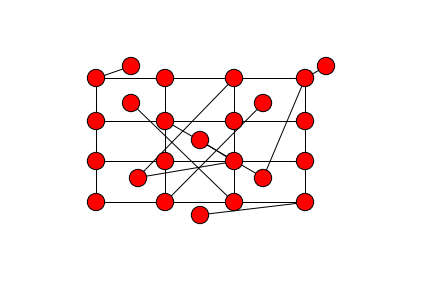
\includegraphics[width = 4.5in]{entiregraph.png}
\end{center}
\end{figure}
\end{frame}
%%%%%%%%%%%%%%%%%%%%%%%%%%%%%%%%%%
\begin{frame}{Graph Partitioning}
\begin{figure}
\begin{center}
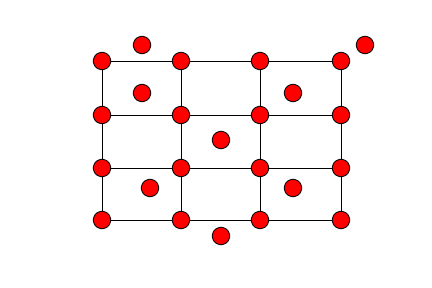
\includegraphics[width = 4in]{planargraph.png}
\caption{Max locally-connected subgraph using Chun-Lu \cite{Chung:2004}}
\end{center}
\end{figure}
\end{frame}


%%%%%%%%%%%%%%%%%%%%%%%%%%%%%%%%%%

\begin{frame}{Linear System Solve}


\begin{figure}
\begin{center}
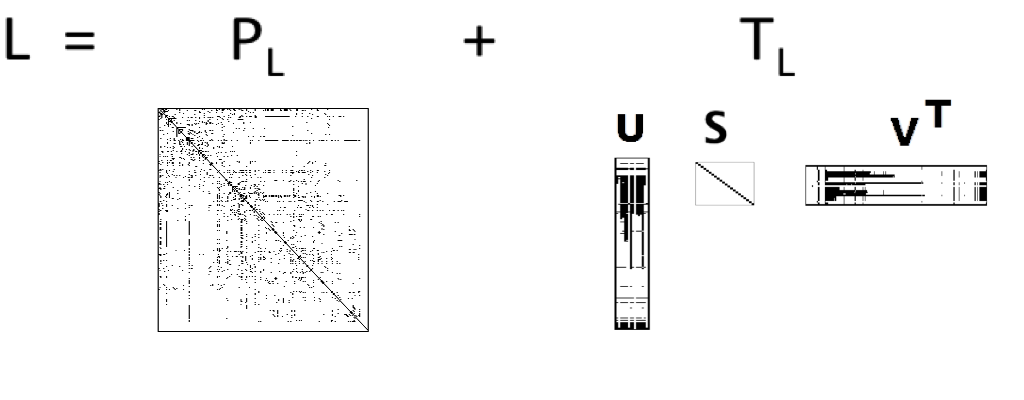
\includegraphics[width = 4.7in]{svd.png}
\end{center}
\end{figure}

\end{frame}
%%%%%%%%%%%%%%%%%%%%%%%%%%%%%%%%%%%%%
\begin{frame}{Linear System Solve}
\begin{Definition}[Sherman-Woodberry-Morrison]
$(P_L + USV^T)^{-1} = P_L^{-1}  - P_L^{-1}U(S^{-1} + V^{T}P_L^{-1}U)^{-1}V^{T}P_L^{-1}$
\end{Definition}
\vspace{.1in}
\begin{align*}
Lx & = b\\
x & = L^{-1}b\\
x & = (P_L+T_L)^{-1}b\\
x & = (P_L+USV)^{-1}b\\
x & = (P_L^{-1}-P_L^{-1}U(S^{-1}+VP_L^{-1}U)^{-1}VP_L^{-1})b\\
x & = P_L^{-1}b-P_L^{-1}U(S^{-1}+VP_L^{-1}U)^{-1}VP_L^{-1}b\\
\end{align*}
\end{frame}

%%%%%%%%%%%%%%%%%%%%%%%%%%%%%%%%%%%%%%

\begin{frame}{Current Solution Approaches}
\large
Multigrid on entire graph: LAMG, CMG, Cascadic
\normalsize
\vspace{.2in}
\begin{itemize}
\item 

How do you coarsen the grid? Based on heuristics

\medskip
\end{itemize}
\vspace{.4in}
\large
Brute force factorization
\normalsize
\vspace{.2in}
\medskip
\begin{itemize}

\item Slow and memory inefficient
\end{itemize}
 

\end{frame}

%%%%%%%%%%%%%%%%%%%%%%%%%%%%%%%%%%%%
\begin{frame}{Partitioning Complexity}
\begin{itemize}
\large
\item
Graph partitioning complexity relies on the degree distribution of the graph
\item
Power law degree graphs with degree sequence:
\begin{center}
\Large
\vspace{.15in}
$P(d) \sim d^{-\gamma}$\\
\vspace{.15in}
$E[d] = \frac{\zeta(\gamma - 1)}{\zeta(\gamma)}$
\end{center}
\vspace{.15in}
\large
\item
Partitioning is $O(iter. \times edges \times E[d]^3)$
\end{itemize}
\end{frame}

%%%%%%%%%%%%%%%%%%%%%%%%%%%%%%%%%%%%

\begin{frame}{Solve Complexity}
\begin{center}
\renewcommand{\arraystretch}{1.5}
    \begin{tabular}{ | l | l |}
    \hline
    \textbf{Operation} & \textbf{O(FLOPs)} \\ \hline
    $USV = T_L$ & $O(n^3)$ \\ \hline
    $S^{-1}$ & $O(r)$ \\ \hline
    $y = P_L^{-1}b$ (MG) & O(n)  \\  \hline
    $y_1 = Vy$ & $O(rn)$ \\ \hline
    $Q = P_L^{-1}U$ ($r$ MG solves) & $O(rn)$ \\ \hline
    $Q_1 = VQ$ & $O(r^2 n)$ \\ \hline
    $Q_2 = S^{-1} + Q_1$ & $O(r^2)$ \\ \hline
    $y_2 = Q_2^{-1}y_1$ & $O(r^3)$ \\ \hline
    $y_3 = Uy_2$ & $O(rn)$ \\ \hline
    $y_4 = P_L^{-1}y_3$ (MG) & $O(n)$ \\ \hline
    $x = y - y_4$ & $O(n)$ \\
    \hline
    \end{tabular}
\end{center}
\end{frame}
%%%%%%%%%%%%%%%%%%%%%%%%%%%%%%%%%%%%%%%%%%

\begin{frame}{Power Law vs. Neural Network Degree Sequence}


\begin{figure}
\begin{center}
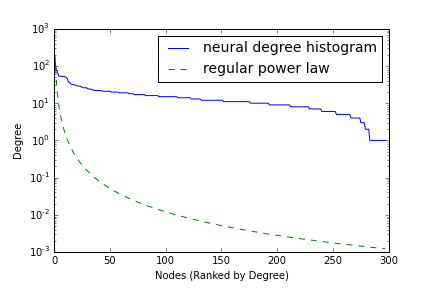
\includegraphics[width=4in]{neuralsequenceplot2.png}
  \caption{$\gamma = 2.1$}
  \end{center}
  \end{figure}

\end{frame}

%%%%%%%%%%%%%%%%%%%%%%%%%%%%%%%%%%%%
\begin{frame}{Stretched Power Law}

\begin{figure}
\begin{center}
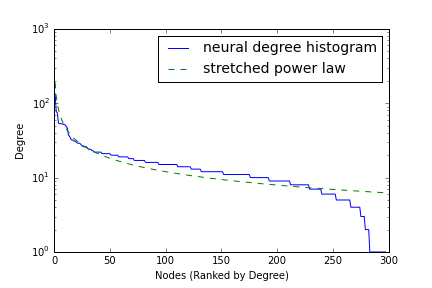
\includegraphics[width=4in]{neuralsequenceplot.png}
\caption{stretched degree is 0.6}
  \end{center}
  \end{figure}

\end{frame}

%%%%%%%%%%%%%%%%%%%%%%%%%%%%%%%%%%%%%%
\begin{frame}{Graphs and Results}
%\begin{center}
\renewcommand{\arraystretch}{1.5}
    \begin{tabular}{| l | l | l | l | l |}
    \hline
    Graph (nodes, edges) & Avg. Deg. & Rank $T_L$ & Part. (s) & Iter. \\ \hline
    Neural (297, 2148) \cite{Watts:1998,White:1986} & 14.46 & 22 & 1.6 & 3 \\ \hline
    Metabolic (453, 2025) \cite{Duch:2005} & 8.94 & 49 & 2.3 & 3 \\  \hline
    Protein (912, 22738) \cite{Simonis:2009} & 49.86 & 26 & 53 & 2 \\ \hline
    Facebook (4039, 88234) \cite{Mcauley:2012} & 43.69 & 180 & 480 & 3 \\ \hline
    Power (4941, 6594) \cite{Watts:1998} & 2.67 & 4284 & .33 & 3\\ 
    \hline
    \end{tabular}
%\end{center}
\end{frame}

%%%%%%%%%%%%%%%%%%%%%%%%%%%%%%%%%%%%%%%%%%%%%
\begin{frame}{Solve Component Results}
These are the limiting solve components according to theoretical complexity and timed results: 

\begin{center}
\renewcommand{\arraystretch}{1.5}
    \begin{tabular}{ | l | l | l | l | l | l | l |}
    \hline
    \textbf{Operation} & \textbf{$O(r,n)$} & \textbf{Neur.} & \textbf{Meta.} & \textbf{Prot.} & \textbf{FB} & \textbf{Pow.} \\ \hline
    $USV = T_L$ & $O(n^3)$ & .0334 & .0737 & .4183 & 38.47 & 72.86  \\ \hline
    %$S^{-1}$ & $O(r)$ & .0005 & .0007 & .0001 & .0023 & 5.104 \\ \hline
    %$y = P_L^{-1}b$ (MG) & $O(n)$ & .0857 & .0962 & .3552 & 1.347 & .1152  \\  \hline
    %$y_1 = Vy$ & $O(rn)$ & .0013 & .0015 & .0002 & .0023 & .0702 \\ \hline
    $Q = P_L^{-1}U$ ($r\times$MG) & $O(rn)$ & .3292 & .7360 & .5190 & 23.11 & 106.9  \\ \hline
    $Q_1 = VQ$ & $O(r^2 n)$ & .0006 & .0036 & .0013 & .4124 & 285.1 \\ \hline
   %$Q_2 = S^{-1} + Q_1$ & $O(r^2)$ & .0012 & .0018 & .0003 & .0011 & .4157 \\ \hline
    $y_2 = Q_2^{-1}y_1$ & $O(r^3)$ & .0023 & .0025 & .0013 & .0099 & 86.49 \\ \hline
    %$y_3 = Uy_2$ & $O(rn)$ & .0001 & .0002 & .0003 & .0025 & .1867 \\ \hline
    %$y_4 = P_L^{-1}y_3$ (MG) & $O(n)$ &.0128 & .0070 & .1183 & .8249 & .0059 \\ \hline
    %$x = y - y_4$ & $O(n)$ &.0003 & .0003 & .0003 & .0004 & .0003 \\ \hline
    \textbf{Total} & \textbf{$O(n^3)$} & \textbf{.51} & \textbf{.966} & \textbf{1.44} & \textbf{64.46} & \textbf{560} \\
    \hline
    \end{tabular}
    \normalsize
\end{center}
\end{frame}


%%%%%%%%%%%%%%%%%%%%%%%%%%%%%%%%%%%%%%%%%%%%%%%%%
\begin{frame}{What Do These Solutions Mean?}
\large
\textit{C. Elegans} data:
\normalsize
\begin{itemize}
\item Important regions in the worm nervous system
\item Key metabolic processes
\item Unobserved protein-phenotype relationships
\end{itemize}
\vspace{.15in}
\large
Facebook friend networks:
\normalsize
\begin{itemize}
\item Origins of influence in a social group
\end{itemize}
\vspace{.15in}
\large
Power Grid:
\normalsize
\begin{itemize}
\item Flow of electricity through urban infrastructure
\end{itemize}
\end{frame}

%%%%%%%%%%%%%%%%%%%%%%%%%%%%%%%%%%%%%%%%%%%%%
\begin{frame}{Conclusions and Future Work}
\begin{itemize}
\item Method to solve the graph laplacian linear system using partitioning and multigrid
\vspace{.15in}
\item Optimize the solve operations and write faster, parallelizable code

\vspace{.15in}
\item Find appropriate linear systems to solve the graphs I have

\vspace{.15in}
\item Test larger graphs; more complex biological systems
\end{itemize}
\end{frame}


%%%%%%%%%%%%%%%%%%%%%%%%%%%%%%%%%%%%%%%%%%%%%%%%%

\begin{frame}{References}
\tiny
\bibliographystyle{plain}
\bibliography{mastersbib}
\end{frame}



\end{document}


